\section{Cross-Validation}
Alle Daten werden fürs Training sowie fürs Testing benutzt und daraus kann das optimale Modell/ Methode für das bestehende Problem ausgewählt werden.
Falls z.B. nur die ersten 75\% fürs Training und die letzten 25\% für Testing verwendet würden, kann nicht garantiert werden ob das Modell wirklich gut ist. In den letzten 25\% könnte es Ausreisser haben, welche das Ergebnis verfälschen würden.\\
\textbf{Problem with 80/20 Data Separation}
\begin{itemize}
    \item Test Error depends on random set
    \item For different Set, the test error would be different
\end{itemize}
With Cross-Validation we can obtain a \textbf{better estimate of the generalization error}

\subsection{k-fold Cross-Validation}
Bei der k-fold Cross-Validation werden die Daten in ''k'' Blöcke (aka Folds) aufgeteilt.\\

\subsubsection{Without k-Fold Cross-Validation}
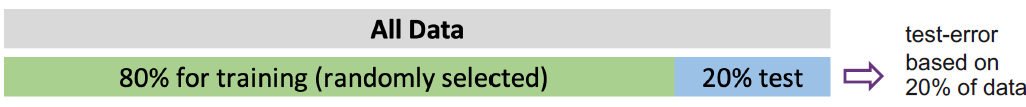
\includegraphics[width=\linewidth]{./img/k_fold.png}

\subsubsection{With k-Fold Cross-Validation}
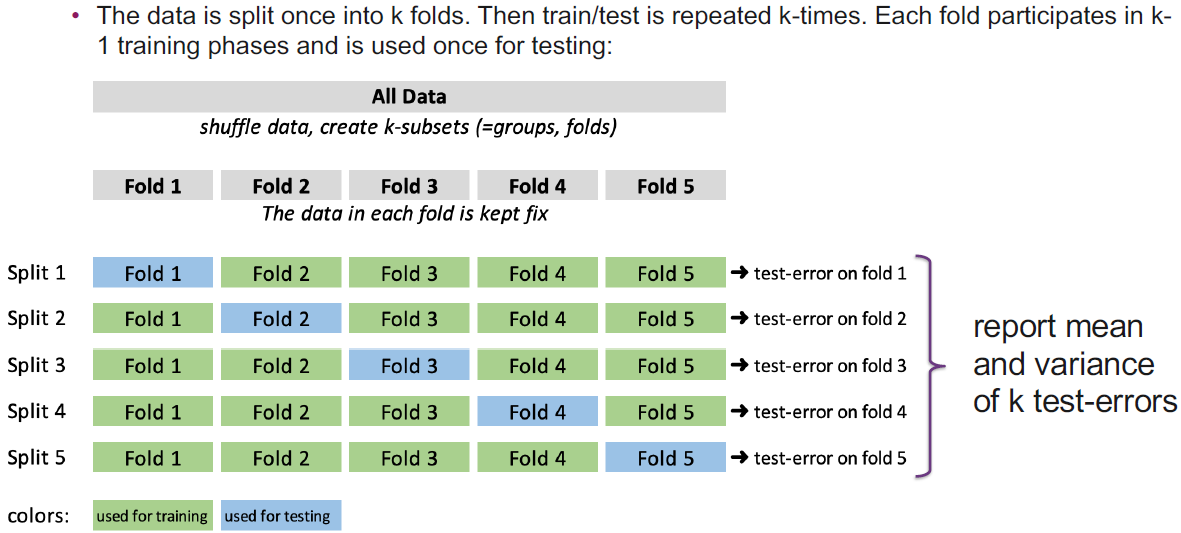
\includegraphics[width=\linewidth]{./img/k_fold2.png}

\subsubsection{Implementation}
\begin{minted}{python}
data = array([1, 2, 3, 4, 5,6]) # data sample
kfold = KFold(n_splits=3, shuffle=True, random_state=1) # prepare cross validation
for train, test in kfold.split(data): # enumerate splits
    print('train: %s, test: %s' % (data[train], data[test]))
# Output:
train: [1, 4, 5, 6], test: [2, 3]
train: [2, 3, 4, 6], test: [1, 5]
train: [1, 2, 3, 5], test: [4, 6]
\end{minted}

\subsubsection{Some Comments}
\begin{itemize}
    \item Typical Values for k are \textit{5,10} or \textit{N}
    \item The data of a fold does not change during procedure
    \item Do not preprocess the whole dataset
    \item Apply the preprocessing pipe-line to each split
\end{itemize}

\section{Artificial Neural Networks (ANN)}
\subsection{Artificial Neurons}
\begin{itemize}
    \item Receives an input vector $[x_1,x_2, ...]$
    \item Each neuron has its own input weights $[w_1, w_2, ...]$ and \textbf{bias} $b$
    \item Calculates the sum of the \textbf{weighted input} (\textit{}{dot product} $\vec{x} * \vec{w}$)
    \item and adds a \textbf{bias} $b$. Then passes the result through a nonlinear activiation function
    \item Be careful when adding more and more neurons to the network: each neuron adds free parameters to the model! We quickly have more parameters than data points, which yields overfitting. 
\end{itemize}
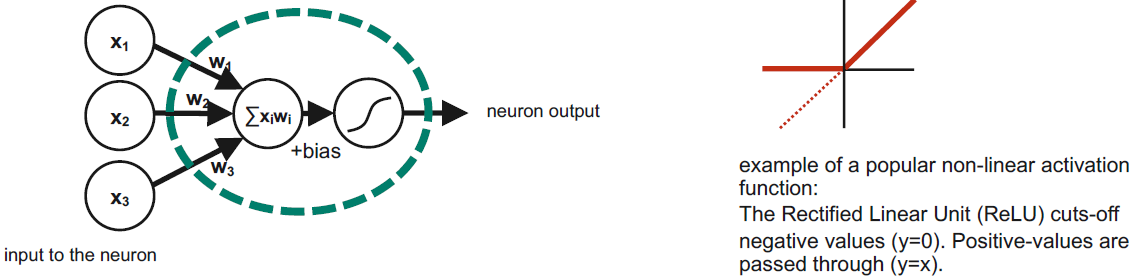
\includegraphics[width=\linewidth]{./img/artificial_neurons.png}

\subsection{Simple ANN}
Computer science definition von ANN:
\begin{itemize}
    \item  ANN ist eine Datenstruktur um eine beliebig komplexe mathematische Formel zu definieren
	\item  ANN ist eine Komposition von relativ simplen Expressions
    \item  ANN ist also wie ein Expression Tree (Root=Output / Leaves=Inputs)
\end{itemize}

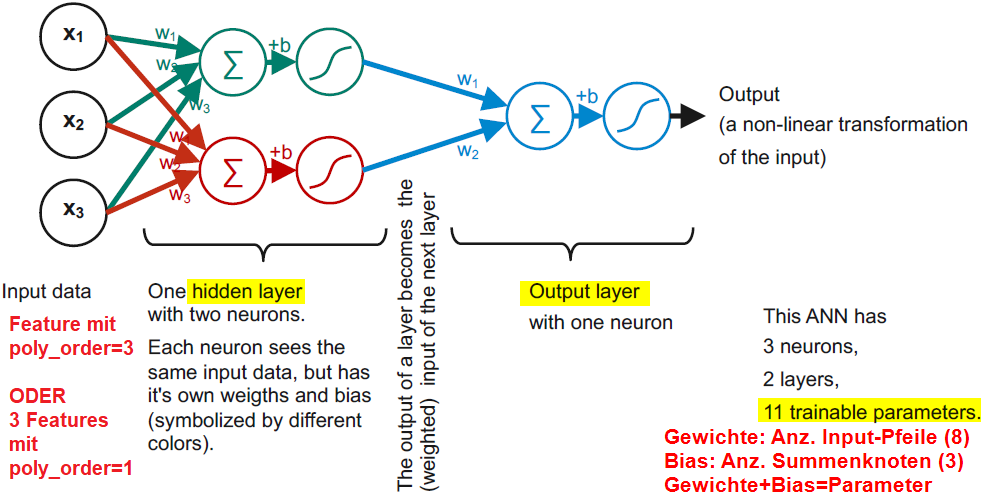
\includegraphics[width=\linewidth]{./img/ann_with_marks.png}
\begin{itemize}
    \item \textbf{Gewicht}: Anzahl Input-Pfeile (hier: 8)
    \item \textbf{Bias}: Anzahl Summenknoten (hier: 3)
    \item \textbf{Trainable Parameters}: Gewicht + Bias (hier: 11)
\end{itemize}

\begin{minted}{python}
poly_order_MODEL = 3 # => order_poly * features = nr of inputs
model = tf.keras.models.Sequential()

# define the input. we provide the dimensionality of the input: poly_order
inputs = keras.Input(shape=(poly_order_MODEL,))
model.add(inputs)

hidden_layer = layers.Dense(2, activation=activations.relu, use_bias=True, kernel_regularizer=regularizers.l2(0.0))
model.add(hidden_layer)

output_layer = layers.Dense(1, activation=activations.relu, use_bias=True, kernel_regularizer=regularizers.l2(0.0))
model.add(output_layer)
\end{minted}
\begin{minted}{text}
--> output
Model: "sequential"
 Layer (type)                Output Shape              Param #   
=================================================================
 dense (Dense)               (None, 2)                 8         
 dense_1 (Dense)             (None, 1)                 3         
=================================================================
Total params: 11
Trainable params: 11
Non-trainable params: 0
\end{minted}

\subsection{Traning an ANN}
\textbf{Supervised learning}
\begin{itemize}
    \item For each input $\vec{x}$ we are given the output $\vec{y}$
    \item ANN is initialized with random weights
    \item An optimizer reduces a cost-function (e.g. MSE)
    \item At every iteration, and for every single weight $w$ and bias $b$, the partial derivative needs to be calculated. (Backpropagation)
\end{itemize}
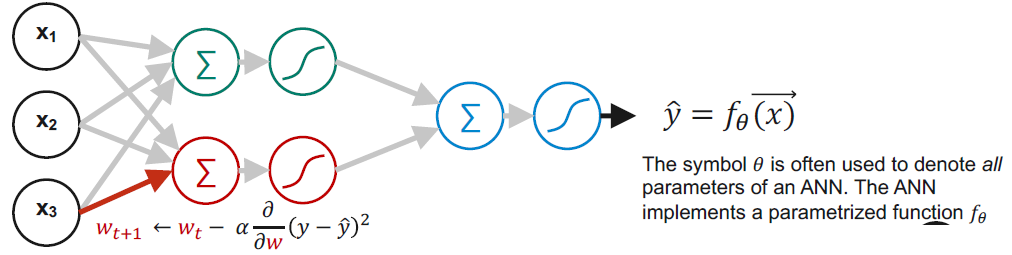
\includegraphics[width=\linewidth]{./img/train_ann.png}

\subsection{Backpropagation}
\begin{itemize}
    \item algorithm is used to effectively train a neural network through a method called chain rule
    \item after each forward pass through a network, backpropagation performs a backward pass while adjusting the model’s parameters (weights and biases)
\end{itemize}

\subsection{Activation Function: ReLu (Rectified Linear Unit)}

\begin{minipage}{0.5\linewidth}
\begin{itemize}
    \item linear function that will output the input directly if \txt{>0}, otherwise it will output 0
    \item default activation function formany types of neural networks, because a model that uses it is easier to train and often achieves better performance
    \item Possible Use Case: when we train the network to learn probabilities (values between 0 and 1)
\end{itemize}
\end{minipage}
\begin{minipage}{0.5\linewidth}
\begin{center}
    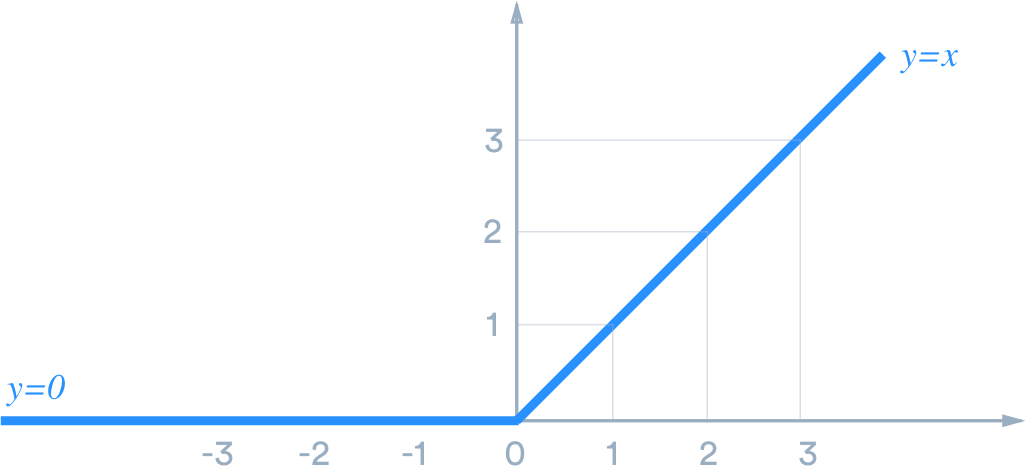
\includegraphics[width=\linewidth]{./img/relu.png}
\end{center}
\end{minipage}




\subsection{Single Input/ Output}
Wenn nur 1 Input vorhanden, dann ist der Input 1-Dimensional (alle Werte passen auf die X-Achse des Diagramms/ Graphen)
\begin{itemize}
    \item X-Achse: Input
    \item Y-Achse: Output
    \item Ergeben zusammen 2-Dimensionalen Graphen (X/Y-Achse)
\end{itemize}

